% !TEX program = pdflatex
% !TEX options = -synctex=1 -interaction=nonstopmode -file-line-error "%DOC%"
% Nonlinear Optics Assignment 4
\documentclass[UTF8,10pt,a4paper]{article}
\usepackage[scheme=plain]{ctex}
\newcommand{\CourseName}{Nonlinear Optics}
\newcommand{\CourseCode}{PHYS2202}
\newcommand{\Semester}{Spring, 2020}
\newcommand{\ProjectName}{Assignment 4}
\newcommand{\DueTimeType}{Due Time}
\newcommand{\DueTime}{17:00, April 15, 2020 (Wednesday)}
\newcommand{\StudentName}{陈稼霖}
\newcommand{\StudentID}{45875852}
\usepackage[vmargin=1in,hmargin=.5in]{geometry}
\usepackage{fancyhdr}
\usepackage{lastpage}
\usepackage{calc}
\pagestyle{fancy}
\fancyhf{}
\fancyhead[L]{\CourseName}
\fancyhead[C]{\ProjectName}
\fancyhead[R]{\StudentName}
\fancyfoot[R]{\thepage\ / \pageref{LastPage}}
\setlength\headheight{12pt}
\fancypagestyle{FirstPageStyle}{
    \fancyhf{}
    \fancyhead[L]{\CourseName\\
        \CourseCode\\
        \Semester}
    \fancyhead[C]{{\Huge\bfseries\ProjectName}\\
        \DueTimeType\ : \DueTime}
    \fancyhead[R]{Name : \makebox[\widthof{\StudentID}][s]{\StudentName}\\
        Student ID\@ : \StudentID\\
        Score : \uline{\makebox[\widthof{\StudentID}]{}}}
    \fancyfoot[R]{\thepage\ / \pageref{LastPage}}
    \setlength\headheight{36pt}
}
\usepackage{amsmath,amssymb,amsthm,bm}
\allowdisplaybreaks[4]
\newtheoremstyle{Problem}
{}
{}
{}
{}
{\bfseries}
{.}
{ }
{\thmname{#1}\thmnumber{ #2}\thmnote{ (#3)} Score: \uline{\qquad\qquad}}
\theoremstyle{Problem}
\newtheorem{prob}{Problem}
\newtheoremstyle{Solution}
{}
{}
{}
{}
{\bfseries}
{:}
{ }
{\thmname{#1}}
\makeatletter
\def\@endtheorem{\qed\endtrivlist\@endpefalse}
\makeatother
\theoremstyle{Solution}
\newtheorem*{sol}{Solution}
\providecommand{\abs}[1]{\left\lvert#1\right\rvert}
\newcommand{\Tr}{\text{Tr }}
\usepackage{ulem}
\usepackage{graphicx}
\usepackage{subfigure}
\begin{document}
\thispagestyle{FirstPageStyle}
\begin{prob}[(25 points) Electromagnetic induced transparency]
    Consider the three-level system represented by the energy diagram below. The excited state, $b$ is much higher in energy relative to the ground state than the thermal energy ($\hbar\omega_{ba}\gg k_BT$) so that we can assume that at equilibrium $\hat{\rho}^{(0)}=\lvert a\rangle\langle a\rvert$. The system is characterized by homogeneous damping rates $\Gamma_{ba}$, $\Gamma_{ca}$, and $\Gamma_{cb}$. Suppose that we use a weak probe pulse at frequency $\omega_p=\omega_{ca}-\delta$ and a strong saturating pump pulse at frequency $\omega_s=c_{cb}-\Delta$. (In other words, the probe and pump beams are detuned from resonance by $\delta$ and $\Delta$ respectively.) Suppose, too, that the detunings are small compared to $\omega_{ba}$: $\delta,\Delta\ll\omega_{ba}$.
    \begin{figure}[h]
        \centering
        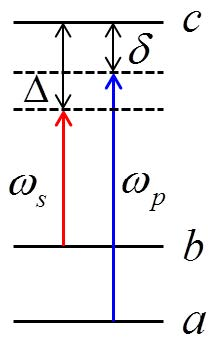
\includegraphics[width=.2\textwidth]{1.jpg}
    \end{figure}
    \begin{enumerate}
        \item[(a)] Using the density-matrix formalism, find the susceptibility associated with the first order \textit{in the probe response}. This requires that we consider the response to infinite order in the pump intensity!\\
        Hint: although we are discussing the frequency domain and so cannot say that one field is present before another, we are interested in the maximally resonant response. If using a diagrammatic approach, think about what that must mean for the ordering of the actual interactions (not simply when the field are present but in what order they must interact). If using a non-diagrammatic approach, pay attention to which terms are fully resonant and which are not.
        \item[(b)] Assume that $\Gamma_{ba}=0.01\Gamma_{ca}=0.01\Gamma_{cb}$. Plot the linear absorption coefficient as a function of probe frequency, $\omega_s$ for $\Delta=0$ in the cases
        \begin{enumerate}
            \item[i.] $\Omega_s=0$ (this is just the normal linear absorption coefficient)
            \item[ii.] $\Omega_s\equiv\abs{\frac{\vec{\mu}_{cb}\cdot\vec{E}_s}{\hbar}}=0.5\Gamma_{ca}$
            \item[iii.] $\Omega_s\equiv\abs{\frac{\vec{\mu}_{cb}\cdot\vec{E}_s}{\hbar}}=5\Gamma_{ca}$
        \end{enumerate}
    \end{enumerate}
\end{prob}
\begin{sol}
    \begin{enumerate}
        \item[(a)] The first order probe response is given by
        \begin{align}
            \langle\hat{\tilde{\bm{p}}}(\omega_p)\rangle=\Tr(\hat{\bm{p}}\hat{\tilde{\rho}}(\omega_p)).
        \end{align}
        In the dipole approximation, $\hat{p}$ has no diagonal elements, so we have
        \begin{align}
            \nonumber\langle\hat{\tilde{\bm{p}}}(\omega_p)\rangle=&\Tr(\hat{\bm{p}}\hat{\tilde{\rho}}(\omega_p))=\sum_{n=a,b,c}\langle n\rvert\hat{\bm{p}}\hat{\tilde{\rho}}(\omega_p)\lvert n\rangle=\sum_{n=a,b,c}\langle n\rvert\hat{\bm{p}}\hat{1}\hat{\tilde{\rho}}(\omega_p)\lvert n\rangle=\sum_{n,m=a,b,c}\langle n\rvert\hat{\bm{p}}\lvert m\rangle\langle m\rvert\hat{\tilde{\rho}}(\omega_p)\lvert n\rangle\\
            =&\uline{\bm{p}_{ab}\tilde{\rho}_{ba}(\omega_p)}+\bm{p}_{ac}\tilde{\rho}_{ca}(\omega_p)+\uline{\bm{p}_{ba}\tilde{\rho}_{ab}(\omega_p)}+\uline{\bm{p}_{bc}\tilde{\rho}_{cb}(\omega_p)}+\uline{\bm{p}_{ca}\tilde{\rho}_{ac}(\omega_p)}+\uline{\bm{p}_{cb}\tilde{\rho}_{bc}(\omega_p)}.
        \end{align}
        The five underlined terms above are actually non-resonant. For example, $\rho_{ba}$ should evolve like $\sim e^{-i(\omega_{ba}+i\Gamma_{ba})t}$, so its component at frequency $\omega_p$, $\tilde{\rho}_{ba}(\omega_p)$ is non-resonant. Neglecting the non-resonant terms, we are left with only one term
        \begin{align}
            \langle\hat{\tilde{\bm{p}}}(\omega')\rangle=\bm{p}_{ac}\tilde{\rho}_{ca}(\omega_p).
        \end{align}
        The Liousville equation for $\rho_{ca}$ is
        \begin{align}
            \label{LE}
            \frac{\partial\rho_{ca}}{\partial t}=-\frac{i}{\hbar}[\hat{H}_0+\hat{H}_I,\hat{\rho}]_{ca}-\Gamma_{ca}\rho_{ca}.
        \end{align}
        The density matrix $\hat{\rho}$ in the time-domain can be expressed as a sum of the Fourier components in the frequency-domain:
        \begin{align}
            \label{FT}
            \hat{\rho}(t)=\sum_j\left[\hat{\tilde{\rho}}(\omega_j)e^{-i\omega_jt}+\text{c.c.}\right],
        \end{align}
        so
        \begin{align}
            \label{FT-1}
            \rho_{ca}(t)=\sum_j\left[\tilde{\rho}_{ca}(\omega_j)e^{-i\omega_jt}+\text{c.c.}\right].
        \end{align}
        Plugging equation \eqref{FT-1} into equation \eqref{LE} and extracting the terms involving $\omega_p$, we get
        \begin{align}
            \label{LE-2}
            -i\omega_p\tilde{\rho}_{ca}(\omega_p)=-\frac{i}{\hbar}[\hat{H}_0,\hat{\rho}]_{ca}(\omega_p)-\frac{i}{\hbar}[\hat{H}_I,\hat{\rho}]_{ca}(\omega_p)-\Gamma_{ca}\rho_{ca}(\omega_p),
        \end{align}
        where $(\omega_p)$ means the component concerning frequency $\omega_p$.\\
        The first term at the right side of equation \eqref{LE-2} is
        \begin{align}
            \label{LE-2-1}
            \nonumber[\hat{H}_0,\hat{\rho}]_{ca}(\omega_p)=&(\hat{H}_0\hat{\rho})_{ca}(\omega_p)-(\hat{\rho}\hat{H}_0)_{ca}(\omega_p)=(\hat{H}_0\hat{1}\hat{\rho})_{ca}(\omega_p)-(\hat{\rho}\hat{1}\hat{H}_0)_{ca}(\omega_p)\\
            \nonumber=&\left(\sum_{m=a,b,c}\hat{H}_0\lvert m\rangle\langle m\rvert\hat{\rho}\right)_{ca}(\omega_p)-\left(\sum_{m=a,b,c}\hat{\rho}\lvert m\rangle\langle m\rvert\hat{H}_0\right)_{ca}(\omega_p)\\
            \nonumber=&\left(\sum_{m=a,b,c}E_m\lvert m\rangle\langle m\rvert\hat{\rho}\right)_{ca}(\omega_p)-\left(\sum_{m=a,b,c}\hat{\rho}\lvert m\rangle\langle m\rvert E_m\right)_{ca}(\omega_p)\\
            \nonumber=&\left(\langle c\rvert\sum_{m=a,b,c}E_m\lvert m\rangle\langle m\rvert\hat{\rho}\lvert a\rangle\right)(\omega_p)-\left(\langle c\rvert\sum_{m=a,b,c}\hat{\rho}\lvert m\rangle\langle m\rvert E_m\lvert a\rangle\right)(\omega_p)\\
            =&E_c\tilde{\rho}_{ca}(\omega_p)-\tilde{\rho}_{ca}(\omega_p)E_a=\hbar\omega_{ca}\tilde{\rho}_{ca}(\omega_p).
        \end{align}
        The second term at the right side of equation \eqref{LE-2} is
        \begin{align}
            \nonumber[\hat{H}_I,\hat{\rho}]_{ca}(\omega_p)=&(\hat{H}_I\hat{\rho})_{ca}(\omega_p)-(\hat{\rho}\hat{H}_I)_{ca}(\omega_p)=(\hat{H}_I\hat{1}\hat{\rho})_{ca}(\omega_p)-(\hat{\rho}\hat{1}\hat{H}_I)_{ca}(\omega_p)\\
            \nonumber=&\left(\sum_{m=a,b,c}\hat{H}_I\lvert m\rangle\langle m\rvert\hat{\rho}\right)_{ca}(\omega_p)-\left(\sum_{m=a,b,c}\hat{\rho}\lvert m\rangle\langle m\rvert\hat{H}_I\right)_{ca}(\omega_p)\\
            \nonumber=&\left(\langle c\rvert\sum_{m=a,b,c}\hat{H}_I\lvert m\rangle\langle m\rvert\hat{\rho}\lvert a\rangle\right)(\omega_p)-\left(\langle c\rvert\sum_{m=a,b,c}\hat{\rho}\lvert m\rangle\langle m\rvert\hat{H}_I\lvert a\rangle\right)(\omega_p)\\
            =&\left(H_{I_{ca}}\rho_{aa}+H_{I_{cb}}\rho_{ba}\right)(\omega_p)-\left(\rho_{cb}H_{I_{ba}}+\rho_{cc}H_{I_{ca}}\right)(\omega_p).
        \end{align}
        The input pulses are at frequencies $\omega_p$ and $\omega_s$, and the complex conjugates are at frequencies $-\omega_p$ and $-\omega_s$, so the Fourier components of the interaction Hamiltonian can only be taken as $\hat{H}_I(\omega_p)$, $\hat{H}_I(\omega_s)$, $\hat{H}_I(-\omega_p)$ and $\hat{H}_I(-\omega_s)$. In this way, the equation above can be factored as
        \small
        \begin{align}
            \nonumber[\hat{H}_I,\hat{\rho}]_{ca}(\omega_p)&=(H_{I_{ca}}\rho_{aa}&&+H_{I_{cb}}\rho_{ba})(\omega_p)&&-(\rho_{cb}H_{I_{ba}}&&+\rho_{cc}H_{I_{ca}})(\omega_p)\\
            \nonumber&=H_{I_{ca}}(\omega_p)\tilde{\rho}_{aa}(0)&&+\uline{H_{I_{cb}}(\omega_p)\tilde{\rho}_{ba}(0)}&&-\uline{\tilde{\rho}_{cb}(0)H_{I_{ba}}(\omega_p)}&&-\uwave{\tilde{\rho}_{cc}(0)H_{I_{ca}}(\omega_p)}\\
            \nonumber&+\uline{H_{I_{ca}}(\omega_s)\tilde{\rho}_{aa}(\omega_p-\omega_s)}&&+H_{I_{cb}}(\omega_s)\tilde{\rho}_{ba}(\omega_p-\omega_s)&&-\uline{\tilde{\rho}_{cb}(\omega_p-\omega_s)H_{I_{ba}}(\omega_s)}&&-\uline{\tilde{\rho}_{cc}(\omega_p-\omega_s)H_{I_{ca}}(\omega_s)}\\
            \nonumber&+\uline{H_{I_{ca}}(-\omega_p)\tilde{\rho}_{aa}(2\omega_p)}&&+\uline{H_{I_{cb}}(-\omega_p)\rho_{ba}(2\omega_p)}&&-\uline{\tilde{\rho}_{cb}(2\omega_p)H_{I_{ba}}(-\omega_p)}&&-\uline{\tilde{\rho}_{cc}(2\omega_p)H_{I_{ca}}(-\omega_p)}\\
            &+\uline{H_{I_{ca}}(-\omega_s)\tilde{\rho}_{aa}(\omega_p+\omega_s)}&&+\uline{H_{I_{cb}}(-\omega_s)\tilde{\rho}_{ba}(\omega_p+\omega_s)}&&-\uline{\tilde{\rho}_{cb}(\omega_p+\omega_s)H_{I_{ba}}(-\omega_s)}&&-\uline{\tilde{\rho}_{cc}(\omega_p+\omega_s)H_{I_{ca}}(-\omega_s)}.
        \end{align}
        \normalsize
        The thirteen underlined terms above are non-resonant. For example, $\rho_{ab}$ should evolve like $\sim e^{-i(\omega_{ab}+i\Gamma_{ba})t}$, so among the four terms involving $\tilde{\rho}_{ba}$, only the component at frequency $\omega_p-\omega_s$, $\tilde{\rho}_{ba}(\omega_p-\omega_s)$ is resonant.\\
        Besides, term $\tilde{\rho}_{cc}H_{I_{ca}}(\omega_p)$ on wavy line is also negligible. Here is the reason: As mentioned in the problem, the energy needed to excite the system from the ground state $a$ to the first excited state $b$ is much higher than the thermal energy, so the initial density matrix of the system at equilibrium is $\lvert a\rangle\langle a\rvert$. To transfer from $\lvert a\rangle\langle a\rvert$, the system has to go through (at least) these interaction processes (just imagining a Feynman diagram in our mind): (1) absorbing a photon at frequency $\omega_p$ from left and a photon at frequency $-\omega_p$ from right so that $\lvert a\rangle\langle a\rvert\longrightarrow\lvert c\rangle\langle c\rvert$, (2) emitting a photon of frequency $-\omega_s$ from left and a photon at frequency $\omega_s$ from right so that $\lvert c\rangle\langle c\rvert\longrightarrow\lvert b\rangle\langle b\rvert$. This whole process involving $2$-order interaction with the probe pulse at frequency $\omega_p$. However, the probe pulse is weak, so we can just omit the terms involving the interactions with the probe pulse at frequency $\omega_p$ higher than $1$-order.\\
        % Since $\omega_p$ is detuned from $\omega_{ca}$ ($\omega_p\approx\omega_{ca}$) and $\omega_s$ is detuned from $\omega_{cb}$ ($\omega_s\approx\omega_{cb}$), to produce resonant contributions to the response, the only possibility is that the system is first excited from state $\lvert a\rangle$ to state $\lvert c\rangle$ by the probe pulse at frequency $\omega_p$ before any other resonant interactions. In this way, any components whose frequency combinations are without $\omega_p$ are non-resonant.\\
        % Also, since the probe pulse is weak, we only focus on terms involving the linear response of the probe pulse. For example, the term $\tilde{\rho}_{aa}(0)=\tilde{\rho}_{aa}(\omega_p-\omega_p)$ refer to the case where the system first interacts with the pulse at frequency $\omega_p$ and then with the pulse at frequency $-\omega_p$. This kind of interaction is $2$-nd order in the probe pulse and is relatively weak.\\
        Neglecting these terms, we are left with only two terms
        \begin{align}
            \label{LE-2-2}
            \nonumber[\hat{H}_I,\hat{\rho}]_{ca}(\omega_p)=&H_{I_{ca}}(\omega_P)\tilde{\rho}_{aa}(0)-\tilde{\rho}_{cc}(0)\hat{H}_{I_{ca}}(\omega_p)+H_{I_{cb}}(\omega_s)\tilde{\rho}_{ba}(\omega_p-\omega_s)\\
            =&[-\bm{p}_{ca}\cdot\bm{E}(\omega_p)]\tilde{\rho}_{aa}(0)+[-\bm{p}_{cb}\cdot\bm{E}(\omega_s)]\tilde{\rho}_{ba}(\omega_p-\omega_s).
        \end{align}
        Plugging equation \eqref{LE-2-1} and equation \eqref{LE-2-2} into equation \eqref{LE-2}, we get
        \begin{align}
            \label{LE-3}
            \boxed{\hbar(\omega_p-\omega_{ca}+i\Gamma_{ca})\tilde{\rho}_{ca}(\omega_p)=-\bm{p}_{ca}\cdot\bm{E}(\omega_p)\tilde{\rho}_{aa}(0)-\bm{p}_{cb}\cdot\bm{E}(\omega_s)\tilde{\rho}_{ba}(\omega_p-\omega_s).}
        \end{align}
        \rule{\columnwidth}{1pt}
        The Liousville equation of \uline{$\rho_{aa}$} is
        \begin{align}
            \frac{\partial\rho_{aa}}{\partial t}=-\frac{i}{\hbar}[\hat{H}_0+\hat{H}_I,\hat{\rho}]_{aa}-\Gamma_{aa}\rho_{aa}.
        \end{align}
        Similarly, plugging equation \eqref{FT} into the above equation and extracting the terms involving frequency $0$, we get
        \begin{align}
            \label{LE-aa-2}
            0=-\frac{i}{\hbar}[\hat{H}_0,\hat{\rho}]_{aa}(0)-\frac{i}{\hbar}[\hat{H}_I,\hat{\rho}]_{aa}(0)-\Gamma_{aa}(\rho_{aa}(0)-1).
        \end{align}
        (Note that the random decay term is $-\Gamma_{11}[\rho_{aa}(0)-\rho_{aa}^0]$ where $\rho_{aa}^0=1$ is the density matrix element at equilibrium.)\\
        The first term at the right side of equation \eqref{LE-aa-2} is
        \begin{align}
            \label{LE-aa-2-1}
            \nonumber[\hat{H}_0,\hat{\rho}]_{aa}(0)=&(\hat{H}_0\hat{\rho})_{aa}(0)-(\hat{\rho}\hat{H}_0)_{aa}(0)=(\hat{H}_0\hat{1}\hat{\rho})_{aa}(0)-(\hat{\rho}\hat{1}\hat{H}_0)_{aa}(0)\\
            \nonumber=&\left(\sum_{m=a,b,c}\hat{H}_0\lvert m\rangle\langle m\rvert\hat{\rho}\right)_{aa}(0)-\left(\sum_{m=a,b,c}\hat{\rho}\lvert m\rangle\langle m\rvert\hat{H}_0\right)_{aa}(0)\\
            \nonumber=&\left(\sum_{m=a,b,c}E_m\lvert m\rangle\langle m\rvert\hat{\rho}\right)_{aa}(0)-\left(\sum_{m=a,b,c}\hat{\rho}\lvert m\rangle\langle m\rvert E_m\right)_{aa}(0)\\
            \nonumber=&\left(\langle a\rvert\sum_{m=a,b,c}E_m\lvert m\rangle\langle m\rvert\hat{\rho}\lvert a\rangle\right)(0)-\left(\langle a\rvert\sum_{m=a,b,c}\hat{\rho}\lvert m\rangle\langle m\rvert E_m\lvert a\rangle\right)(0)\\
            =&E_a\tilde{\rho}_{aa}(0)-\tilde{\rho}_{aa}(0)E_a=0.
        \end{align}
        The second term at the right side of equation \eqref{LE-aa-2} is
        \begin{align}
            \nonumber[\hat{H}_I,\hat{\rho}]_{aa}(0)=&(\hat{H}_I\hat{\rho})_{aa}(0)-(\hat{\rho}\hat{H}_I)_{aa}(0)=(\hat{H}_I\hat{1}\hat{\rho})_{aa}(0)-(\hat{\rho}\hat{1}\hat{H}_I)_{aa}(0)\\
            \nonumber=&\left(\sum_{m=a,b,c}\hat{H}_I\lvert m\rangle\langle m\rvert\hat{\rho}\right)_{aa}(0)-\left(\sum_{m=a,b,c}\hat{\rho}\lvert m\rangle\langle m\rvert\hat{H}_I\right)_{aa}(0)\\
            \nonumber=&\left(\langle a\rvert\sum_{m=a,b,c}\hat{H}_I\lvert m\rangle\langle m\rvert\hat{\rho}\lvert a\rangle\right)(0)-\left(\langle a\rvert\sum_{m=a,b,c}\hat{\rho}\lvert m\rangle\langle m\rvert\hat{H}_I\lvert a\rangle\right)(0)\\
            \nonumber=&(H_{I_{ab}}\rho_{ba}+H_{I_{ac}}\rho_{ca})(0)-(\rho_{ab}H_{I_{ba}}+\rho_{ac}H_{I_{ca}})(0)
        \end{align}
        \begin{align}
            \nonumber&=\uline{H_{I_{ab}}(\omega_p)\tilde{\rho}_{ba}(-\omega_p)}&&+\uline{H_{I_{ac}}(\omega_p)\tilde{\rho}_{ca}(-\omega_p)}&&-\uline{\tilde{\rho}_{ab}(-\omega_p)H_{I_{ba}}(\omega_p)}&&-\uwave{\tilde{\rho}_{ac}(-\omega_p)H_{I_{ca}}(\omega_p)}\\
            \nonumber&+\uline{H_{I_{ab}}(\omega_s)\tilde{\rho}_{ba}(-\omega_s)}&&+\uline{H_{I_{ac}}(\omega_s)\tilde{\rho}_{ca}(-\omega_s)}&&-\uline{\tilde{\rho}_{ab}(-\omega_s)H_{I_{ba}}(\omega_s)}&&-\uline{\tilde{\rho}_{ac}(-\omega_s)H_{I_{ca}}(\omega_s)}\\
            \nonumber&+\uline{H_{I_{ab}}(-\omega_p)\tilde{\rho}_{ba}(\omega_p)}&&+\uwave{H_{I_{ac}}(-\omega_p)\tilde{\rho}_{ca}(\omega_p)}&&-\uline{\tilde{\rho}_{ab}(\omega_p)H_{I_{ba}}(-\omega_p)}&&-\uline{\tilde{\rho}_{ac}(\omega_p)H_{I_{ca}}(-\omega_p)}\\
            &+\uline{H_{I_{ab}}(-\omega_s)\tilde{\rho}_{ba}(\omega_s)}&&+\uline{H_{I_{ac}}(-\omega_s)\tilde{\rho}_{ca}(\omega_s)}&&-\uline{\tilde{\rho}_{ab}(\omega_s)H_{I_{ba}}(-\omega_s)}&&-\uline{\tilde{\rho}_{ac}(\omega_s)H_{I_{ca}}(-\omega_s)}.
        \end{align}
        The fourteen underlined terms are non-resonant. The two terms on wavy lines involves the density matrix elements oscillating at $\pm\omega_p$ (so there must have already been an interaction with the probe pulse) and then interacting with the field at frequency $\mp\omega_p$ again. Since the probe pulse at frequency $\omega_p$ is weak, these $2$-order interaction terms are negligible. Neglecting the non-resonant terms and the terms involving $2$-order interactions with the probe pulse, we find that the above equation is equal to zero:
        \begin{align}
            \label{LE-aa-2-2}
            [\hat{H}_I,\hat{\rho}]_{aa}(0)=0.
        \end{align}
        Plugging equation \eqref{LE-aa-2-1} and equation \eqref{LE-aa-2-2} to equation \eqref{LE-aa-2}, we get
        \begin{align}
            \label{LE-aa-3}
            \boxed{\tilde{\rho}_{aa}(0)=1.}
        \end{align}
        % \rule{\columnwidth}{1pt}
        % The Liousville equation of \uline{$\rho_{cc}$} is
        % \begin{align}
        %     \frac{\partial\rho_{cc}}{\partial t}=-\frac{i}{\hbar}[\hat{H}_0+\hat{H}_I,\hat{\rho}]_{cc}-\Gamma_{cc}\rho_{cc}.
        % \end{align}
        % Plugging equation \eqref{FT} into the above equation and extracting the terms involving frequency $0$, we get
        % \begin{align}
        %     \label{LE-cc-2}
        %     0=-\frac{i}{\hbar}[\hat{H}_0,\hat{\rho}]_{cc}(0)-\frac{i}{\hbar}[\hat{H}_I,\hat{\rho}]_{cc}(0)-\Gamma_{cc}\rho_{cc}(0).
        % \end{align}
        % The first term at the right side of equation \eqref{LE-cc-2} is
        % \begin{align}
        %     \label{LE-cc-2-1}
        %     \nonumber[\hat{H}_0,\hat{\rho}]_{cc}(0)=&(\hat{H}\hat{\rho})_{cc}(0)-(\hat{\rho}\hat{H}_0)_{cc}(0)=(\hat{H}\hat{1}\hat{\rho})_{cc}(0)-(\hat{\rho}\hat{1}\hat{H}_0)_{cc}(0)\\
        %     \nonumber=&\left(\sum_{m=a,b,c}\hat{H}_0\lvert m\rangle\langle m\rvert\hat{\rho}\right)_{cc}(0)-\left(\sum_{m=a,b,c}\hat{\rho}\lvert m\rangle\langle m\rvert\hat{H}_0\right)_{cc}(0)\\
        %     \nonumber=&\left(\sum_{m=a,b,c}E_m\lvert m\rangle\langle m\rvert\hat{\rho}\right)_{cc}(0)-\left(\sum_{m=a,b,c}\hat{\rho}\lvert m\rangle\langle m\rvert E_m\right)_{cc}(0)\\
        %     \nonumber=&\left(\langle c\rvert\sum_{m=a,b,c}E_m\lvert m\rangle\langle m\rvert\hat{\rho}\lvert c\rangle\right)(0)-\left(\langle c\rvert\sum_{m=a,b,c}\hat{\rho}\lvert m\rangle\langle m\rvert E_m\lvert c\rangle\right)(0)\\
        %     =&E_c\tilde{\rho}_{cc}(0)-\tilde{\rho}_{cc}(0)E_c=0.
        % \end{align}
        % The second term at the right side of equation \eqref{LE-cc-2} is
        % \begin{align}
        %     \nonumber[\hat{H}_I,\hat{\rho}]_{cc}(0)=&(\hat{H}_I\hat{\rho})_{cc}(0)-(\hat{\rho}\hat{H}_I)_{cc}(0)=(\hat{H}_I\hat{1}\hat{\rho})_{cc}(0)-(\hat{\rho}\hat{1}\hat{H}_I)_{cc}(0)\\
        %     \nonumber=&\left(\sum_{m=a,b,c}\hat{H}_I\lvert m\rangle\langle m\rvert\hat{\rho}\right)_{cc}(0)-\left(\sum_{m=a,b,c}\hat{\rho}\lvert m\rangle\langle m\rvert\hat{H}_I\right)_{cc}(0)\\
        %     \nonumber=&\left(\langle c\rvert\sum_{m=a,b,c}\hat{H}_I\lvert m\rangle\langle m\rvert\hat{\rho}\lvert c\rangle\right)(0)-\left(\langle c\rvert\sum_{m=a,b,c}\hat{\rho}\lvert m\rangle\langle m\rvert\hat{H}_I\lvert c\rangle\right)(0)\\
        %     \nonumber=&(H_{I_{ca}}\rho_{ac}+H_{I_{cb}}\rho_{bc})(0)-(\rho_{ca}\hat{H}_{I_{ac}}+\rho_{cb}\hat{H}_{I_{bc}})(0)
        % \end{align}
        % \begin{align}
        %     \nonumber&=\uwave{H_{I_{ca}}(\omega_p)\tilde{\rho}_{ac}(-\omega_p)}&&+\uline{H_{I_{cb}}(\omega_p)\tilde{\rho}_{bc}(-\omega_p)}&&-\uline{\tilde{\rho}_{ca}(-\omega_p)H_{ac}(\omega_p)}&&-\uline{\tilde{\rho}_{cb}(-\omega_p)\hat{H}_{I_{bc}}(\omega_p)}\\
        %     \nonumber&+\uline{H_{I_{ca}}(\omega_s)\tilde{\rho}_{ac}(-\omega_s)}&&+H_{I_{cb}}(\omega_s)\tilde{\rho}_{bc}(-\omega_s)&&-\uline{\tilde{\rho}_{ca}(-\omega_s)H_{ac}(\omega_s)}&&-\uline{\tilde{\rho}_{cb}(-\omega_s)\hat{H}_{I_{bc}}(\omega_s)}\\
        %     \nonumber&+\uline{H_{I_{ca}}(-\omega_p)\tilde{\rho}_{ac}(\omega_p)}&&+\uline{H_{I_{cb}}(-\omega_p)\tilde{\rho}_{bc}(\omega_p)}&&-\uwave{\tilde{\rho}_{ca}(\omega_p)H_{ac}(-\omega_p)}&&-\uline{\tilde{\rho}_{cb}(\omega_p)\hat{H}_{I_{bc}}(-\omega_p)}\\
        %     &+\uline{H_{I_{ca}}(-\omega_s)\tilde{\rho}_{ac}(\omega_s)}&&+\uline{H_{I_{cb}}(-\omega_s)\tilde{\rho}_{bc}(\omega_s)}&&-\uline{\tilde{\rho}_{ca}(\omega_s)H_{ac}(-\omega_s)}&&-\tilde{\rho}_{cb}(\omega_s)\hat{H}_{I_{bc}}(-\omega_s).
        % \end{align}
        % The twelve underlined terms are non-resonant and the two terms on wavy lines involving $2$nd-order interaction with the probe pulse. Neglecting these terms, we are left with only two terms
        % \begin{align}
        %     \label{LE-cc-2-2}
        %     \nonumber[\hat{H}_I,\hat{\rho}]_{aa}(0)=&H_{I_{cb}}(\omega_s)\tilde{\rho}_{bc}(-\omega_s)-\tilde{\rho}_{cb}(\omega_s)\hat{H}_{I_{bc}}(-\omega_s)\\
        %     =&[-\bm{p}_{cb}\cdot\bm{E}(\omega_s)]\tilde{\rho}_{bc}(-\omega_s)-\tilde{\rho}_{cb}(\omega_s)[-\bm{p}_{bc}\cdot\bm{E}(-\omega_s)].
        % \end{align}
        % Plugging equation \eqref{LE-cc-2-1} and equation \eqref{LE-cc-2-2} into equation \eqref{LE-cc-2}, we get
        % \begin{align}
        %     \label{LE-cc-3}
        %     \boxed{i\hbar\Gamma_{cc}\tilde{\rho}_{cc}(0)=-\bm{p}_{cb}\cdot\bm{E}(\omega_s)\tilde{\rho}_{bc}(-\omega_s)+\bm{p}_{bc}\cdot\bm{E}^*(\omega_s)\tilde{\rho}_{cb}(\omega_s).}
        % \end{align}
        \rule{\columnwidth}{1pt}
        The Liousville equation of \uline{$\rho_{ba}$} is
        \begin{align}
            \frac{\partial\rho_{ba}}{\partial t}=-\frac{i}{\hbar}[\hat{H}_0+\hat{H}_I,\hat{\rho}]_{ba}-\Gamma_{ba}\rho_{ba}.
        \end{align}
        Plugging equation \eqref{FT} into the above equation and extracting the terms involving frequency $\omega_p-\omega_s$, we get
        \begin{align}
            \label{LE-ba-2}
            -i(\omega_p-\omega_s)\tilde{\rho}_{ba}(\omega_p-\omega_s)=-\frac{i}{\hbar}[\hat{H}_0,\hat{\rho}]_{ba}(\omega_p-\omega_s)-\frac{i}{\hbar}[\hat{H}_I,\hat{\rho}]_{ba}(\omega_p-\omega_s)-\Gamma_{ba}\rho_{ba}(\omega_p-\omega_s).
        \end{align}
        The first term at the right side of equation \eqref{LE-ba-2} is
        \begin{align}
            \label{LE-ba-2-1}
            \nonumber[\hat{H}_0,\hat{\rho}]_{ba}(\omega_p-\omega_s)=&(\hat{H}_0\hat{\rho})_{ba}(\omega_p-\omega_s)-(\hat{\rho}\hat{H}_0)_{ba}(\omega_p-\omega_s)=(\hat{H}_0\hat{1}\hat{\rho})_{ba}(\omega_p-\omega_s)-(\hat{\rho}\hat{1}\hat{H}_0)_{ba}(\omega_p-\omega_s)\\
            \nonumber=&\left(\sum_{m=a,b,c}\hat{H}_0\lvert m\rangle\langle m\rvert\hat{\rho}\right)_{ba}(\omega_p-\omega_s)-\left(\sum_{m=a,b,c}\hat{\rho}\lvert m\rangle\langle m\rvert\hat{H}_0\right)_{ba}(\omega_p-\omega_s)\\
            \nonumber=&\left(\sum_{m=a,b,c}E_m\lvert m\rangle\langle m\rvert\hat{\rho}\right)_{ba}(\omega_p-\omega_s)-\left(\sum_{m=a,b,c}\hat{\rho}\lvert m\rangle\langle m\rvert E_m\right)_{ba}(\omega_p-\omega_s)\\
            \nonumber=&\left(\langle b\rvert\sum_{m=a,b,c}E_m\lvert m\rangle\langle m\rvert\hat{\rho}\lvert a\rangle\right)(\omega_p-\omega_s)-\left(\langle b\rvert\sum_{m=a,b,c}\hat{\rho}\lvert m\rangle\langle m\rvert E_m\rvert a\rangle\right)(\omega_p-\omega_s)\\
            =&E_b\tilde{\rho}_{ba}(\omega_p-\omega_s)-\tilde{\rho}_{ba}(\omega_p-\omega_s)E_a=\hbar\omega_{ba}\tilde{\rho}_{ba}(\omega_p-\omega_s).
        \end{align}
        The second term at the right side of equation \eqref{LE-ba-2} is
        \begin{align}
            \nonumber[\hat{H}_I,\hat{\rho}]_{ba}(\omega_p-\omega_s)=&(\hat{H}_I\hat{\rho})_{ba}(\omega_p-\omega_s)-(\hat{\rho}\hat{H}_I)_{ba}(\omega_p-\omega_s)=(\hat{H}_I\hat{1}\hat{\rho})_{ba}(\omega_p-\omega_s)-(\hat{\rho}\hat{1}\hat{H}_I)_{ba}(\omega_p-\omega_s)\\
            \nonumber=&\left(\sum_{m=a,b,c}\hat{H}_I\lvert m\rangle\langle m\rvert\hat{\rho}\right)_{ba}(\omega_p-\omega_s)-\left(\sum_{m=a,b,c}\hat{\rho}\lvert m\rangle\langle m\rvert\hat{H}_I\right)_{ba}(\omega_p-\omega_s)\\
            \nonumber=&\left(\langle b\rvert\sum_{m=a,b,c}\hat{H}_I\lvert m\rangle\langle m\rvert\hat{\rho}\lvert a\rangle\right)(\omega_p-\omega_s)-\left(\langle b\rvert\sum_{m=a,b,c}\hat{\rho}\lvert m\rangle\langle m\rvert\hat{H}_I\lvert a\rangle\right)(\omega_p-\omega_s)\\
            \nonumber=&(H_{I_{ba}}\tilde{\rho}_{aa}+H_{I_{bc}}\tilde{\rho}_{ca})(\omega_p-\omega_s)-(\tilde{\rho}_{bb}H_{I_{ba}}+\tilde{\rho}_{bc}H_{I_{ca}})(\omega_p-\omega_s)
        \end{align}
        \begin{align}
            \nonumber&=\uline{H_{I_{ba}}(\omega_p)\tilde{\rho}_{aa}(-\omega_s)}&&+\uline{H_{I_{bc}}(\omega_p)\tilde{\rho}_{ca}(-\omega_s)}&&-\uline{\tilde{\rho}_{bb}(-\omega_s)H_{I_{ba}}(\omega_p)}&&-\uwave{\tilde{\rho}_{bc}(-\omega_s)H_{I_{ca}}(\omega_p)}\\
            \nonumber&+\uline{H_{I_{ba}}(\omega_s)\tilde{\rho}_{aa}(\omega_p-2\omega_s)}&&+\uline{H_{I_{bc}}(\omega_s)\tilde{\rho}_{ca}(\omega_p-2\omega_s)}&&-\uline{\tilde{\rho}_{bb}(\omega_p-2\omega_s)H_{I_{ba}}(\omega_s)}&&-\uline{\tilde{\rho}_{bc}(\omega_p-2\omega_s)H_{I_{ca}}(\omega_s)}\\
            \nonumber&+\uline{H_{I_{ba}}(-\omega_p)\tilde{\rho}_{aa}(2\omega_p-\omega_s)}&&+\uline{H_{I_{bc}}(-\omega_p)\tilde{\rho}_{ca}(2\omega_p-\omega_s)}&&-\uline{\tilde{\rho}_{bb}(2\omega_p-\omega_s)H_{I_{ba}}(-\omega_p)}&&-\uline{\tilde{\rho}_{bc}(2\omega_p-\omega_s)H_{I_{ca}}(-\omega_p)}\\
            &+\uline{H_{I_{ba}}(-\omega_s)\tilde{\rho}_{aa}(\omega_p)}&&+H_{I_{bc}}(-\omega_s)\tilde{\rho}_{ca}(\omega_p)&&-\uline{\tilde{\rho}_{bb}(\omega_p)H_{I_{ba}}(-\omega_s)}&&-\uline{\tilde{\rho}_{bc}(\omega_s)H_{I_{ca}}(-\omega_s)}.
        \end{align}
        The fourteen underlined terms are non-resonant and the one term on wavy line involves $2$-order interaction with the probe pulse. Neglecting these terms, we are left with only two term
        \begin{align}
            \label{LE-ba-2-2}
            \nonumber[\hat{H}_I,\hat{\rho}]_{ba}(\omega_p-\omega_s)=&H_{I_{bc}}(-\omega_s)\tilde{\rho}_{ca}(\omega_p)\\
            =&[-\bm{p}_{bc}\cdot\bm{E}(-\omega_s)]\tilde{\rho}_{ca}(\omega_p).
        \end{align}
        Plugging equation \eqref{LE-ba-2-1} and \eqref{LE-ba-2-2} into equation \eqref{LE-ba-2}, we get
        \begin{align}
            \label{LE-ba-3}
            \boxed{\hbar(\omega_p-\omega_s-\omega_{ba}+i\Gamma_{ba})\tilde{\rho}_{ba}(\omega_p-\omega_s)=-\bm{p}_{bc}\cdot\bm{E}^*(\omega_s)\tilde{\rho}_{ca}(\omega_p).}
        \end{align}
        % \rule{\columnwidth}{1pt}
        % The Liousville equation of \uline{$\rho_{cb}$} is
        % \begin{align}
        %     \frac{\partial\rho_{cb}}{\partial t}=-\frac{i}{\hbar}[\hat{H}_0+\hat{H}_I,\hat{\rho}]_{cb}-\Gamma_{cb}\rho_{cb}.
        % \end{align}
        % Plugging equation \eqref{FT} into the above equation and extracting the terms involving frequency $\omega_s$, we get
        % \begin{align}
        %     \label{LE-cb-2}
        %     -i\omega_s\tilde{\rho}_{cb}(\omega_s)=-\frac{i}{\hbar}[\hat{H}_0,\hat{\rho}]_{cb}(\omega_s)-\frac{i}{\hbar}[\hat{H}_I,\hat{\rho}]_{cb}(\omega_s)-\Gamma_{cb}\tilde{\rho}_{cb}(\omega_s).
        % \end{align}
        % The first term at the right side of equation \eqref{LE-cb-2} is
        % \begin{align}
        %     \label{LE-cb-2-1}
        %     \nonumber[\hat{H}_0,\hat{\rho}]_{cb}(\omega_s)=&(\hat{H}_0\hat{\rho})_{cb}(\omega_s)-(\hat{\rho}\hat{H}_0)_{cb}(\omega_s)=(\hat{H}_0\hat{1}\hat{\rho})_{cb}(\omega_s)-(\hat{\rho}\hat{1}\hat{H}_0)_{cb}(\omega_s)\\
        %     \nonumber=&\left(\sum_{m=a,b,c}\hat{H}_0\lvert m\rangle\langle m\rvert\hat{\rho}\right)_{cb}(\omega_s)-\left(\sum_{m=a,b,c}\hat{\rho}\lvert m\rangle\langle m\rvert\hat{H}_0\right)_{cb}(\omega_s)\\
        %     \nonumber=&\left(\sum_{m=a,b,c}E_m\lvert m\rangle\langle m\rvert\hat{\rho}\right)_{cb}(\omega_s)-\left(\sum_{m=a,b,c}\hat{\rho}\lvert m\rangle\langle m\rvert E_m\right)_{cb}(\omega_s)\\
        %     \nonumber=&\left(\langle c\rvert\sum_{m=a,b,c}E_m\lvert m\rangle\langle m\rvert\hat{\rho}\lvert b\rangle\right)(\omega_s)-\left(\langle c\rvert\sum_{m=a,b,c}\hat{\rho}\lvert m\rangle\langle m\rvert E_m\lvert b\rangle\right)(\omega_s)\\
        %     =&E_c\tilde{\rho}_{cb}(\omega_s)-\tilde{\rho}_{cb}(\omega_s)E_b=\hbar\omega_{cb}\tilde{\rho}_{cb}(\omega_s).
        % \end{align}
        % The second term at the right side of equation \eqref{LE-cb-2} is
        % \begin{align}
        %     \nonumber[\hat{H}_I,\hat{\rho}]_{cb}(\omega_s)=&(\hat{H}_0\hat{\rho})_{cb}(\omega_s)-(\hat{\rho}\hat{H}_I)_{cb}(\omega_s)=(\hat{H}_0\hat{1}\hat{\rho})_{cb}(\omega_s)-(\hat{\rho}\hat{1}\hat{H}_I)_{cb}(\omega_s)\\
        %     \nonumber=&\left(\sum_{m=a,b,c}\hat{H}_0\lvert m\rangle\langle m\rvert\hat{\rho}\right)_{cb}(\omega_s)-\left(\sum_{m=a,b,c}\hat{\rho}\lvert m\rangle\langle m\rvert\hat{H}_I\right)_{cb}(\omega_s)\\
        %     \nonumber=&\left(\langle c\rvert\sum_{m=a,b,c}\hat{H}_0\lvert m\rangle\langle m\rvert\hat{\rho}\lvert b\rangle\right)(\omega_s)-\left(\langle c\rvert\sum_{m=a,b,c}\hat{\rho}\lvert m\rangle\langle m\rvert\hat{H}_I\lvert b\rangle\right)(\omega_s)\\
        %     \nonumber=&(H_{ca}\rho_{ab}+H_{cb}\rho_{bb})(\omega_s)-(\rho_{ca}H_{I_{ab}}+\rho_{cc}\hat{H}_{I_{cb}})(\omega_s)
        % \end{align}
        % \begin{align}
        %     \nonumber&=\uwave{H_{I_{ca}}(\omega_p)\tilde{\rho}_{ab}(\omega_s-\omega_p)}&&+\uline{H_{I_{cb}}(\omega_p)\tilde{\rho}_{bb}(\omega_s-\omega_p)}&&-\uline{\tilde{\rho}_{ca}(\omega_s-\omega_p)H_{I_{ab}}(\omega_p)}&&-\tilde{\rho}_{cc}(\omega_s-\omega_p)\hat{H}_{I_{cb}}(\omega_p)\\
        %     \nonumber&+\uline{H_{I_{ca}}(\omega_s)\tilde{\rho}_{ab}(0)}&&+H_{I_{cb}}(\omega_s)\tilde{\rho}_{bb}(0)&&-\uline{\tilde{\rho}_{ca}(0)H_{I_{ab}}(\omega_s)}&&-\uline{\tilde{\rho}_{cc}(0)\hat{H}_{I_{cb}}(\omega_s)}\\
        %     \nonumber&+\uline{H_{I_{ca}}(-\omega_p)\tilde{\rho}_{ab}(\omega_p+\omega_s)}&&+\uline{H_{I_{cb}}(-\omega_p)\tilde{\rho}_{bb}(\omega_p+\omega_s)}&&-\uline{\tilde{\rho}_{ca}(\omega_p+\omega_s)H_{I_{ab}}(-\omega_p)}&&-\uline{\tilde{\rho}_{cc}(\omega_p+\omega_s)\hat{H}_{I_{cb}}(-\omega_p)}\\
        %     &+\uline{H_{I_{ca}}(-\omega_s)\tilde{\rho}_{ab}(2\omega_s)}&&+\uline{H_{I_{cb}}(-\omega_s)\tilde{\rho}_{bb}(2\omega_s)}&&-\uline{\tilde{\rho}_{ca}(2\omega_s)H_{I_{ab}}(-\omega_s)}&&-\uline{\tilde{\rho}_{cc}(2\omega_s)\hat{H}_{I_{cb}}(-\omega_s)}.
        % \end{align}
        % The thirteen underlined terms above are non-resonant and the one term on wavy line involves $2$-nd order interaction with the probe pulse. Neglecting these terms, we are left with only two terms
        % \begin{align}
        %     \label{LE-cb-2-2}
        %     \nonumber[\hat{H}_I,\hat{\rho}]_{cb}(\omega_s)=&H_{I_{cb}}(\omega_s)\tilde{\rho}_{bb}(0)-\tilde{\rho}_{cc}(0)H_{I_{cb}}(\omega_s)\\
        %     =&[-\bm{p}_{cb}\cdot\bm{E}(\omega_s)]\tilde{\rho}_{bb}(0)-\tilde{\rho}_{cc}(0)[-\bm{p}_{cb}\cdot\bm{E}(\omega_s)].
        % \end{align}
        % Plugging equation \eqref{LE-cb-2-1} and equation \eqref{LE-cb-2-2} into equation \eqref{LE-cb-2}, we get
        % \begin{align}
        %     \label{LE-cb-3}
        %     \boxed{\hbar(\omega_s-\omega_{cb}+i\Gamma_{cb})\tilde{\rho}_{cb}(\omega_s)=\bm{p}_{cb}\cdot\bm{E}(\omega_s)[\tilde{\rho}_{cc}(0)-\tilde{\rho}_{bb}(0)].}
        % \end{align}
        % Using the fact that $\tilde{\rho}_{cb}(\omega_s)$ and $\tilde{\rho}(-\omega_s)$ are complex conjugates, $\tilde{\rho}_{cb}(\omega_s)^*=\tilde{\rho}_{bc}(-\omega_s)$, we have
        % \begin{align}
        %     \label{LE-bc}
        %     \boxed{\hbar(\omega_s-\omega_{cb}-i\Gamma_{cb})\tilde{\rho}_{bc}(\omega_s)=\bm{p}_{bc}\cdot\bm{E}^*(\omega_s)[\tilde{\rho}_{cc}(0)-\tilde{\rho}_{bb}(0)].}
        % \end{align}
        % \rule{\columnwidth}{1pt}
        % The Liousville equation of \uline{$\rho_{bb}$} is
        % \begin{align}
        %     \frac{\partial\rho_{bb}}{\partial t}=-\frac{i}{\hbar}[\hat{H}_0+\hat{H}_I,\hat{\rho}]_{bb}-\Gamma_{bb}\rho_{bb}.
        % \end{align}
        % Plugging equation \eqref{FT} into the above equation and extracting the terms involving frequency $0$, we get
        % \begin{align}
        %     \label{LE-bb-2}
        %     0=-\frac{i}{\hbar}[\hat{H}_0,\hat{\rho}]_{bb}(0)-\frac{i}{\hbar}[\hat{H}_I,\hat{\rho}]_{bb}(0)-\Gamma_{bb}\tilde{\rho}_{bb}(0).
        % \end{align}
        % The first term at the right side of equation \eqref{LE-bb-2} is
        % \begin{align}
        %     \label{LE-bb-2-1}
        %     \nonumber[\hat{H}_0,\hat{\rho}]_{bb}=&(\hat{H}_0\hat{\rho})_{bb}(0)-(\hat{\rho}\hat{H}_0)_{bb}(0)=(\hat{H}_0\hat{1}\hat{\rho})_{bb}(0)-(\hat{\rho}\hat{1}\hat{H}_0)_{bb}(0)\\
        %     \nonumber=&\left(\sum_{m=a,b,c}\hat{H}_0\lvert m\rangle\langle m\rvert\hat{\rho}\right)_{bb}(0)-\left(\sum_{m=a,b,c}\hat{\rho}\lvert m\rangle\langle m\rvert\hat{H}_0\right)_{bb}(0)\\
        %     \nonumber=&\left(\sum_{m=a,b,c}E_m\lvert m\rangle\langle m\rvert\hat{\rho}\right)_{bb}(0)-\left(\hat{\rho}\lvert m\rangle\langle m\rvert E_m\right)_{bb}(0)\\
        %     \nonumber=&\left(\langle b\rvert\sum_{m=a,b,c}E_m\lvert m\rangle\langle m\rvert\hat{\rho}\lvert b\rangle\right)(0)-\left(\sum_{m=a,b,c}\langle b\rvert\hat{\rho}\lvert m\rangle\langle m\rvert E_m\lvert b\rangle\right)(0)\\
        %     =&E_b\tilde{\rho}_{bb}(0)-\tilde{\rho}_{bb}(0)E_b=0
        % \end{align}
        % The second term at the right side of equation \eqref{LE-bb-2} is
        % \begin{align}
        %     \nonumber[\hat{H}_I,\hat{\rho}]_{bb}=&(\hat{H}_I\hat{\rho})_{bb}(0)-(\hat{\rho}\hat{H}_I)_{bb}(0)=(\hat{H}_I\hat{1}\hat{\rho})_{bb}(0)-(\hat{\rho}\hat{1}\hat{H}_I)_{bb}(0)\\
        %     \nonumber=&\left(\sum_{m=a,b,c}\hat{H}_I\lvert m\rangle\langle m\rvert\hat{\rho}\right)_{bb}(0)-\left(\sum_{m=a,b,c}\hat{\rho}\lvert m\rangle\langle m\rvert\hat{H}_I\right)_{bb}(0)\\
        %     \nonumber=&\left(\langle b\rvert\sum_{m=a,b,c}\hat{H}_I\lvert m\rangle\langle m\rvert\hat{\rho}\lvert m\rangle\right)(0)-\left(\langle b\rvert\sum_{m=a,b,c}\hat{\rho}\lvert m\rangle\langle m\rvert\hat{H}_I\lvert b\rangle\right)(0)\\
        %     \nonumber=&(H_{I_{ba}}\rho_{ab}+H_{I_{bc}}\rho_{cb})(0)-(\rho_{ba}\hat{H}_{I_{ab}}+\rho_{bc}\hat{H}_{I_{cb}})(0)
        % \end{align}
        % \begin{align}
        %     \nonumber&=\uline{H_{I_{ba}}(\omega_p)\tilde{\rho}_{ab}(-\omega_p)}&&+\uline{H_{I_{bc}}(\omega_p)\tilde{\rho}_{cb}(-\omega_p)}&&-\uline{\tilde{\rho}_{ba}(-\omega_p)H_{I_{ab}}(\omega_p)}&&-\uline{\tilde{\rho}_{bc}(-\omega_p)H_{I_{cb}}(\omega_p)}\\
        %     \nonumber&+\uline{H_{I_{ba}}(\omega_s)\tilde{\rho}_{ab}(-\omega_s)}&&+\uline{H_{I_{bc}}(\omega_s)\tilde{\rho}_{cb}(-\omega_s)}&&-\uline{\tilde{\rho}_{ba}(-\omega_s)H_{I_{ab}}(\omega_s)}&&-\tilde{\rho}_{bc}(-\omega_s)H_{I_{cb}}(\omega_s)\\
        %     \nonumber&+\uline{H_{I_{ba}}(-\omega_p)\tilde{\rho}_{ab}(\omega_p)}&&+\uline{H_{I_{bc}}(-\omega_p)\tilde{\rho}_{cb}(\omega_p)}&&-\uline{\tilde{\rho}_{ba}(\omega_p)H_{I_{ab}}(-\omega_p)}&&-\uline{\tilde{\rho}_{bc}(\omega_p)H_{I_{cb}}(-\omega_p)}\\
        %     &+\uline{H_{I_{ba}}(-\omega_s)\tilde{\rho}_{ab}(\omega_s)}&&+H_{I_{bc}}(-\omega_s)\tilde{\rho}_{cb}(\omega_s)&&-\uline{\tilde{\rho}_{ba}(\omega_s)H_{I_{ab}}(-\omega_s)}&&-\uline{\tilde{\rho}_{bc}(\omega_s)H_{I_{cb}}(-\omega_s)}.
        % \end{align}
        % The fourteen underlined terms are non-resonant. Neglecting these terms, we are left with only two terms
        % \begin{align}
        %     \label{LE-bb-2-2}
        %     \nonumber[\hat{H}_I,\hat{\rho}]_{bb}=&-\tilde{\rho}_{bc}(-\omega_s)H_{I_{cb}}(\omega_s)+H_{I_{bc}}(-\omega_s)\tilde{\rho}_{cb}(\omega_s)\\
        %     =&-\tilde{\rho}_{bc}(-\omega_s)[-\bm{p}_{cb}\cdot\bm{E}(\omega_s)]+[-\bm{p}_{bc}\cdot\bm{E}(-\omega_s)]\tilde{\rho}_{cb}(\omega_s).
        % \end{align}
        % Plugging equation \eqref{LE-bb-2-1} and equation \eqref{LE-bb-2-2} into equation \eqref{LE-bb-2}, we get
        % \begin{align}
        %     \label{LE-bb-3}
        %     \boxed{i\hbar\Gamma_{bb}\tilde{\rho}_{bb}(0)=\bm{p}_{cb}\cdot\bm{E}(\omega_s)\tilde{\rho}_{bc}(-\omega_s)-\bm{p}_{bc}\cdot\bm{E}^*(\omega_s)\tilde{\rho}_{cb}(\omega_s).}
        % \end{align}
        % \rule{\columnwidth}{1pt}
        % Using equation \eqref{LE-cc-3}, equation \eqref{LE-cb-3}, equation \eqref{LE-bc}, equation \eqref{LE-bb-3}, we get
        % \begin{align}
        %     \tilde{\rho}_{cc}(0)=0.
        % \end{align}
        \rule{\columnwidth}{1pt}
        Plugging equation \eqref{LE-aa-3} and equation\eqref{LE-ba-3} into equation \eqref{LE-3} (these are the three boxed Liousville equation), we get
        \begin{align}
            \nonumber&\tilde{\rho}_{ca}(\omega_p)=\frac{-\bm{p}_{ca}\cdot\bm{E}(\omega_p)}{\hbar(\omega_p-\omega_{ca}+i\Gamma_{ca})-\frac{\abs{\bm{p}_{cb}\cdot\bm{E}(\omega_s)}^2}{\hbar(\omega_p-\omega_s-\omega_{ba}+i\Gamma_{ba})}}\\
            =&\frac{\bm{p}_{ca}\cdot\bm{E}(\omega_p)}{\hbar}\frac{1}{(\omega_p-\omega_s-\omega_{ba}-i\Gamma_{ba})\frac{\Omega_s^2}{(\omega_p-\omega_s-\omega_{ba})^2+\Gamma_{ba}^2}-(\omega_p-\omega_{ca}+i\Gamma_{ca})}.
        \end{align}
        where $\Omega_s\equiv\frac{\abs{\bm{p}_{cb}\cdot\bm{E}(\omega_s)}}{\hbar}$.\\
        The first order probe response is
        \begin{align}
            \langle\hat{\tilde{\rho}}(\omega_p)\rangle=\bm{p}_{ac}\tilde{\rho}_{ca}(\omega_p)=\frac{\bm{p}_{ac}[\bm{p}_{ca}\cdot\bm{E}(\omega_p)]}{\hbar}\frac{1}{(\omega_p-\omega_s-\omega_{ba}-i\Gamma_{ba})\frac{\Omega_s^2}{(\omega_p-\omega_s-\omega_{ba})^2+\Gamma_{ba}^2}-(\omega_p-\omega_{ca}+i\Gamma_{ca})}.
        \end{align}
        The susceptibility associated with it is
        \begin{align}
            \nonumber&\chi^{(1)}(\omega_p)=\frac{N\langle\hat{\tilde{\rho}}(\omega_p)\rangle}{\varepsilon_0\bm{E}(\omega_p)}=\frac{N\abs{\bm{p}_{ca}}^2}{\varepsilon_0\hbar}\frac{1}{(\omega_p-\omega_s-\omega_{ba}-i\Gamma_{ba})\frac{\Omega_s^2}{(\omega_p-\omega_s-\omega_{ba})^2+\Gamma_{ba}^2}-(\omega_p-\omega_{ca}+i\Gamma_{ca})}\\
            \nonumber=&\frac{N\abs{\bm{p}_{ca}}^2}{\varepsilon_0\hbar}[(\omega_p-\omega_s-\omega_{ba})^2+\Gamma_{ba}^2]\times\\
            &\qquad\qquad\frac{\left\{(\omega_p-\omega_s-\omega_{ba})\Omega_s^2-(\omega_p-\omega_{ca})[(\omega_p-\omega_s-\omega_{ba})^2+\Gamma_{ba}^2]\right\}+i\left\{\Gamma_{ba}\Omega_s^2+\Gamma_{ca}[(\omega_p-\omega_s-\omega_{ba})^2+\Gamma_{ba}^2]\right\}}{\left\{(\omega_p-\omega_s-\omega_{ba})\Omega_s^2-(\omega_p-\omega_{ca})[(\omega_p-\omega_s-\omega_{ba})^2+\Gamma_{ba}^2]\right\}^2+\left\{\Gamma_{ba}\Omega_s^2+\Gamma_{ca}[(\omega_p-\omega_s-\omega_{ba})^2+\Gamma_{ba}^2]\right\}^2}.
        \end{align}
        where $N$ the number density of the atoms.
        \item[(b)] When $\Delta=0$, the susceptibility is
        \begin{align}
            \nonumber&\chi^{(1)}(\omega_p)\\
            =&\frac{N\abs{\bm{p}_{ca}}^2}{\varepsilon_0\hbar}[(\omega_p-\omega_{ca})^2+\Gamma_{ba}^2]\times\frac{(\omega_p-\omega_{ca})\left\{\Omega_s^2-[(\omega_p-\omega_{ca})^2+\Gamma_{ba}^2]\right\}+i\left\{\Gamma_{ba}\Omega_s^2+\Gamma_{ca}[(\omega_p-\omega_{ca})^2+\Gamma_{ba}^2]\right\}}{(\omega_p-\omega_{ca})^2\left\{\Omega_s^2-[(\omega_p-\omega_{ca})^2+\Gamma_{ba}^2]\right\}^2+\left\{\Gamma_{ba}\Omega_s^2+\Gamma_{ca}[(\omega_p-\omega_{ca})^2+\Gamma_{ba}^2]\right\}^2}.
        \end{align}
        The linear absorption coefficient is
        \begin{align}
            \nonumber&\alpha(\omega_p)=2\frac{\omega_p}{c}\text{Im }\sqrt{1+\chi^{(1)}(\omega_p)}\approx\frac{\omega_p}{c}\text{Im }\chi^{(1)}(\omega_p)\\
            =&\frac{N\abs{\bm{p}_{ca}}^2\omega_p}{\varepsilon_0\hbar c}[(\omega_p-\omega_{ca})^2+\Gamma_{ba}^2]\times\frac{\left\{\Gamma_{ba}\Omega_s^2+\Gamma_{ca}[(\omega_p-\omega_{ca})^2+\Gamma_{ba}^2]\right\}}{(\omega_p-\omega_{ca})^2\left\{\Omega_s^2-[(\omega_p-\omega_{ca})^2+\Gamma_{ba}^2]\right\}^2+\left\{\Gamma_{ba}\Omega_s^2+\Gamma_{ca}[(\omega_p-\omega_{ca})^2+\Gamma_{ba}^2]\right\}^2}
        \end{align}
        We set $\Gamma_{ca}=1.0$, $\omega_{ca}=10.0$.
        \begin{enumerate}
            \item[i.] If $\Omega_s=0$, the linear absorption coefficient as a function of the probe pulse $\omega_p$ is shown in figure \ref{AbsorptionCoefficient-1}.
            \item[ii.] If $\Omega_s=0.5\Gamma_{ca}$, the linear absorption coefficient as a function of the probe pulse $\omega_p$ is shown in figure \ref{AbsorptionCoefficient-2}.
            \item[iii.] If $\Omega_s=5\Gamma_{ca}$, the linear absorption coefficient as a function of the probe pulse $\omega_p$ is shown in figure \ref{AbsorptionCoefficient-3}.
            \begin{figure}[h]
                \centering
                \subfigure[$\Omega_s=0$.]{
                \label{AbsorptionCoefficient-1}
                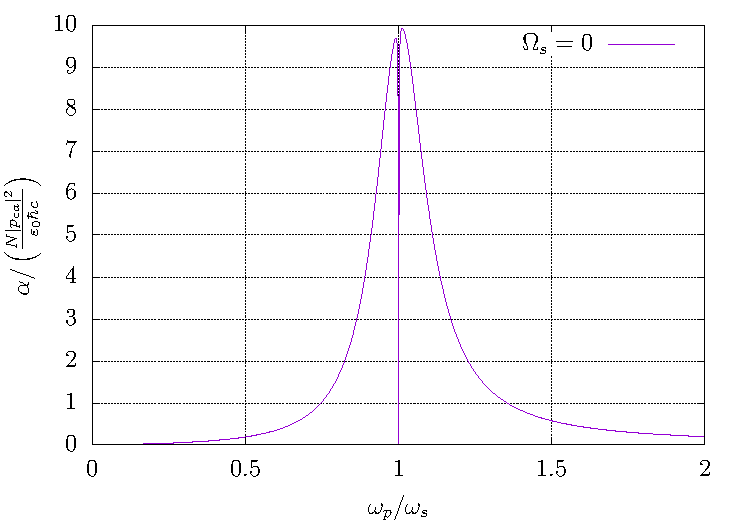
\includegraphics[width=.6\textwidth]{AbsorptionCoefficient-1.pdf}}
                \subfigure[$\Omega_s=0.5\Gamma_{ca}$.]{
                \label{AbsorptionCoefficient-2}
                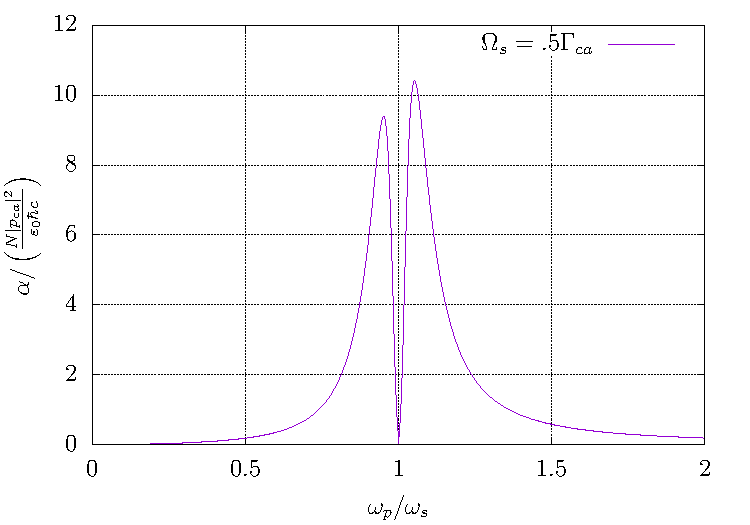
\includegraphics[width=.6\textwidth]{AbsorptionCoefficient-2.pdf}}
                \subfigure[$\Omega_s=5\Gamma_{ca}$.]{
                \label{AbsorptionCoefficient-3}
                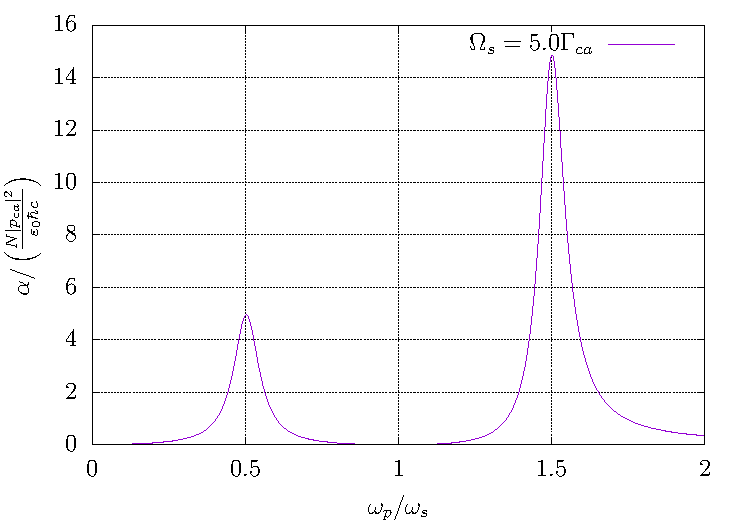
\includegraphics[width=.6\textwidth]{AbsorptionCoefficient-3.pdf}}
                \caption{The absorption coefficient.}
            \end{figure}
        \end{enumerate}
    \end{enumerate}
\end{sol}
\end{document}